\section{Background and Introduction}
\label{sec:intro}  

\section*{Introduction: A reconfigurable reinforcement learning method}

\subsection{RLN MDP structure}
\label{sec:rlnmdpstructure}

The general approach that is taken to form an RLN is ``split'' one single MDP into parent and child processes. Doing so assumes the two process are partly independent [CMDP]. 

\begin{enumerate}[label=\arabic*.]
\item Largely, the models may be independent.
\item The child and parent may include elements of each other's MDP definition in their own definition.
\end{enumerate}

This section focuses on framing a model. In Sections~\ref{sec:mapping} and later, subjects related to behavior optimality, convergence, and computational complexity are considered.

In order to consider the formation of a reconfigurable reinforcement network, it is required to analytically group all aspects of a process and a behavior policy into one tuples.

\begin{center}
\scalebox{0.5}{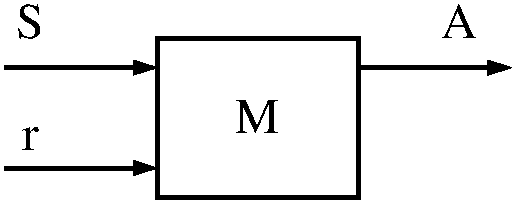
\includegraphics{media/page4diagram.pdf}}
\end{center}

To do this, assume a Markov decision process M which can be internally modeled as a tuple \( M = \langle S, A, T, R, \pi, \tilde{T}, \tilde{R}\rangle \)\\

$S$ -- a set of states $s\in S$ which may be experienced by $M$\\
$A$ -- a set of actions $a\in A$ that may be executed\\
$T$ -- a true transitional probability, $T(s^{\prime}|a,s)$ expressing the probability of executing an action $a$ in state $s$ before ending up in later state $s^{\prime}$.\\
$R$ -- is a reward function which quantifies how desirable a transition $R(s'|a,s)$ is. $R: S\times A \times S\rightarrow \mathbb{R}_{\geq 0}$\\
$\tilde{T}$ -- is the current model of $T$. The goal of $\tilde{T}$ is thus $\tilde{T}\sim T$\\
$\tilde{R}$ -- is the predicted reward of the system, constructed from observation of $R$, s.t.\ $\tilde{R}\rightarrow R$. \\
$\pi$ -- is an action selection policy, ideally chosen to maximize expected reward, an optimal policy is denoted $\pi^*$. Ideally
\begin{equation*}
\pi^*(s) = \argmax_{a}\sum_{s^\prime}\underbrace{R(s^\prime|a,s) T(s'|a,s)+\gamma V(s^\prime)}_{\text{expected reward}}
\end{equation*}
and
\begin{equation*}
\tilde{\pi}(s)  = \argmax_{a}\sum_{s^\prime}\tilde{R}(s^\prime|a,s) \tilde{T}(s'|a,s)+\gamma \tilde{V}(s^\prime)
\end{equation*}

\textbf{[Note that $\tilde{V}$ hasn't been defined in the previous equation.]}

\section*{encoding}

\begin{equation*}
\pi^*(s) = \argmax_{a}\sum_{s^\prime} R(s^\prime|s,a) T(s'|s,a)+\gamma V(s^\prime)
\end{equation*}
where
\begin{equation*}
V(s) = \sum_{s^\prime} R(s^\prime|s,a) T(s^\prime|s,a) +V(s^\prime)\,.
\end{equation*}
A bellman backup can be used [Bellman backup]. In online applications stochastic gradient descent can be applied to regress to locally optimal solutions. This allows estimation of optimal policy
\begin{equation*}
\pi^*(s) = \argmax_{a} Q(s,a)\,.
\end{equation*}

To encode the expected reward over all states, typically $Q$-values are kept: $ Q(s,a) \sim \sum R(s^\prime|a,s)T(s^\prime|a,s)+\gamma V(s^\prime) $ and $ Q_{t+1}(s,a) \leftarrow Q_t(s,a)+\alpha \left( R(s^\prime|a,s)-Q_t(s,a)+\gamma\argmax_{a^\prime} Q(s^\prime,a^\prime) \right) $.

To render the process $M$ separable, it is necessary to decouple the transitional values $T$ from the reward values $R$. Thus, to directly encode $Q(s,a)$ using $\pi$ is prohibitive.\\
knowing: 
\begin{equation*}
Q: S \times A \to \mathbb{R}_{\geq 0}
\end{equation*}
indirect encoding:
\begin{equation*}
\pi: \left\{ S \times A \times S \times \mathbb{N} \middle| R \right\} \to Q
\end{equation*}
If the definitions of $S$ or $A$ change, then $Q$ must be reinitialized. Alternatively, $\tilde{T}$ and $\tilde{R}$ are defined as intermediate encoding functions. Thus we define
\begin{equation*}
\pi:\left\{S \times A \times S \times \mathbb{N}\right\} \to \tilde{T}, \tilde{R}, Q
\end{equation*} 
simple transition
\begin{equation*}
\tilde{T}_{t+1}(s^\prime|s,a) = \frac{\textrm{freq}(s^\prime|s,a)}{\textrm{freq}(s,a)}
\end{equation*}
simple reward
\begin{equation*}
\tilde{R}_{t+1}(s^\prime|s,a) = \tilde{R}(s^\prime|s,a)+\alpha_R\left( \tilde{R}(s^\prime|s,a)-R(s^\prime|s,a)\right)
\end{equation*}
\begin{equation*}
f_Q: \tilde{T}_t \times \tilde{R}_t \to Q_t
\end{equation*}
In this paper we rely on a method of extracting dynamic $Q$-values from an encoded transition and reward function $( \tilde{T}, \tilde{R} )$. The motivation for this encoding is that it allows mapping the transition function into multiple spaces, and allows the reward function to be altered. The significance of this finding is covered in \textbf{???} Price wash \textbf{???}.

  
\subsection{Reconfiguration of $M$}

Reconfiguring a process $M$ allows some intractable MDPs to be rendered tractable. 
As an example, take an MDP $M$ modeling a 3-dimensional foraging experiment with three thousand positions on the $x$, $y$, and $z$
axes respectively. This process will consume over three billion memory locations and may be impossible to explore. If this system is
broken into three sub problems, each targeting a special axis, then only nine thousand memory locations need be consumed. This decreases memory requirements by an exponential factor.

This section presents a method of decomposition that, when followed, introduces no degeneration of the regressed policy $\pi^{*}(s,a)$.
The summary of these conditions is presented. There is no free lunch: the trade-off for saving in space is exponentially increased computational burden. As in all problems, finding the balance between space and computational complexity is required.

 

\subsubsection{Introduction to approach}

The general approach is related to factor analysis, or clustering, eigenvalue decomposition, or projected component analysis, with which the reader may be familiar. The process is split such that a subspace $S_i \subseteq S$, and action space $A_i \subseteq A$ seem independent of subspaces $S_k$, $A_k$, for the purposes of generating reward $R(s^\prime|a,s)$. Specifically, it may be observed that the reward is homogeneous, such that 
\begin{equation*}
\forall k_2, a_2: R\left(S^\prime_i \cup  S^\prime_{k_1} \middle| S_i \cup S_{k_1} , a_i \cup a_{k_1} \right) \sim R\left( S^\prime_i \cup S^\prime_{k_2}  \middle|  S_i \cup S_{k_2} , a_i \cup a_{k_2}  \right)\,.
\end{equation*}
In this case, it is likely that the problem may be separated. Even in the case where variance of reward is high, convergence is expected.

Splitting is done using a decomposition function
\begin{equation*}
d^{M_i,M_k}_{M} = M \longrightarrow \left\{    M_i, M_k \middle|
\begin{array}{l}
S_i \times ( S_k / \{s_i\} ) = S, S_k \times ( S_i / \{ s_k \} ) = S \\
A=A_i \cup A_k\\
\tilde{T}\sim d^{-1}(d(\tilde{T})),d(\tilde{T})=\tilde{T}_i, \tilde{T}_k\\
\tilde{R}\sim d^{-1}(d(\tilde{R})), d(\tilde{R})=\tilde{R}_i,\tilde{R}_k
\end{array}
 \right\}
\end{equation*}
where $d$ represents belief mapping functions that decompose and recompose $\tilde{T}$ and $\tilde{R}$. This allows  $M$ to be mapped as new spaces and observations are encountered. The decomposition process breaks one MDP into a parent and child:\\

\begin{center}
\scalebox{0.5}{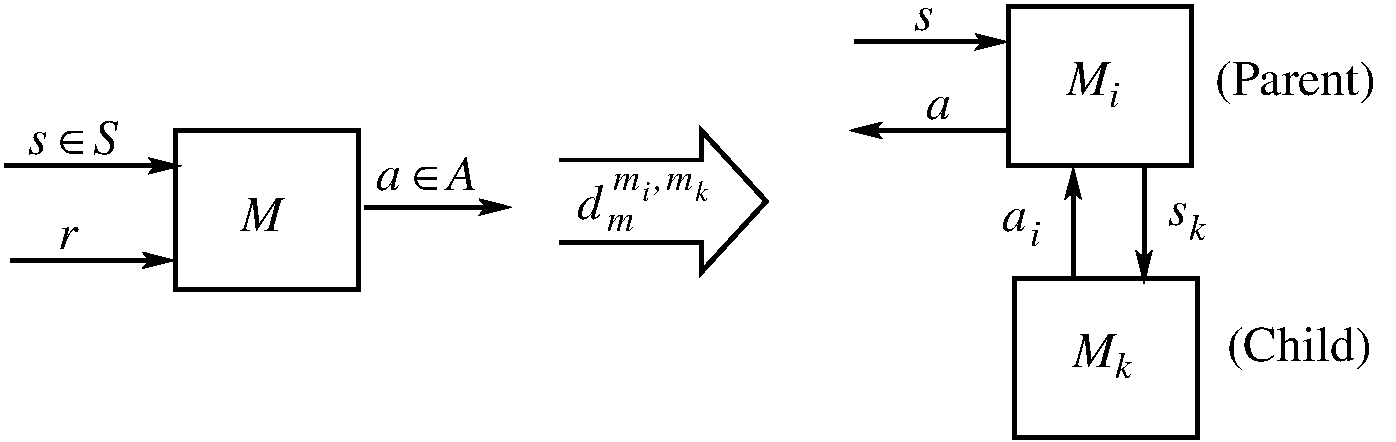
\includegraphics{media/page5figure}}
\end{center}


\newpage


Although many decomposition strategies are possible, this work presents a specific approach related to parent--child decomposition. This specific decomposition allows for assured policy convergence (see Section~\ref{})

\underline{Definitions}\\

\underline{$M$}\quad
\begin{minipage}[t]{5in}
$S=(S_i/S_k)\times(S_k/S_i)$\\
$A=A_i\cup A_k$\\
$T=P(S\times A\times S)$\\
$R= \text{real, positive, convergent stochastic as $t\to\infty$}$\\
$R(s^\prime,a,s) =R\left( 
\begin{array}{c} s^\prime_i \\ s^\prime_k \end{array},
\begin{array}{c} a_i \\ a_k \end{array},
\begin{array}{c} s_i \\ s_k \end{array}
\right)$
\end{minipage}\\

The system can be broken into the following MDP definitions

\underline{$M_i$ -- Parent}\\

$S_i$ -- a collection of states, $s_i\in S_i$\\
$A_i$ -- a collection of actions, $a_i \in A_i$\\
$\tilde{T}( s^\prime_i | s_i, a_i )$ -- the observed probability of executing action $a_i$ in state $s_i$ and ending up in state $s^\prime_i$\\

\begin{equation*}
\left. \begin{array}{l}
\tilde{T}\\
\tilde{R}
\end{array}\right\}
\text{Covered Pages on BII p12-14}
\end{equation*}

$P(s^\prime_i|s_i, a_i)$ is observed directly and is $\tilde{T}( s^\prime_i | s_i, a_i )$\\

%$R_t\left({}^{s^\prime_i}_{a^\prime_k}|{}_{a_i},{}^{s_i}_{a_k}\right)=R_t\left({}^{s^\prime_i}_{s^\prime_k},{}^{a_i}_{a_k},{}^{s_i}_{s_k}\right)$

\begin{equation*}
\tilde{R}_t\left(  \begin{array}{l} s^\prime_i \\ a^\prime_k \end{array}
\middle| 
\begin{array}{c}  a_i \\ \end{array},
\begin{array}{c} s_i \\ a_k \end{array}
\right) 
=
\tilde{R}_t\left( 
\begin{array}{c} s^\prime_i \\ s^\prime_k \end{array}, \middle|
\begin{array}{c} a_i \\ a_k \end{array},
\begin{array}{c} s_i \\ s_k \end{array}
\right)
=
\tilde{R}( s^\prime | a, s )
\end{equation*}


$S$, $T_i$, $S_k$, $S^\prime_k$ are not directly observable by process $M_i$, by design. Importantly, some facts are known about $a_k$ and $a^\prime_k$ which will be exploited in Section~\ref{}.\\

ii) $a_k=\pi_k(s_k)$\\
iii) $a^\prime_k=\pi_k(s_k)$\\
iiii) $\left(s_k,s^\prime_k\right)$ chosen indirectly by $\pi_k(\cdot)$ in a manner that assuming monotonic increase in reward,
\begin{equation*}
  \text{as\ }t \to \infty \quad E[R_{t+1}(\cdot)] \geq E[R_t(\cdot)]\,.
\end{equation*}
Local convergence of this process on a behavior policy $\pi^*_i(\cdot)$ is assured.

\underline{$M_k$ -- child}\\

$S^\prime_i$ -- all child states, $s_k\in S_k$\\
$a_k\in A_k$\\
$\tilde{T}(s^\prime_k|s_k,a_k)$\\
$R_t(s^\prime_k,a_k,s_k)=R_t\left({}^{s_i}_{s^\prime_k},{}^{a_i}_{a_k},{}^{s_i}_{s_k}\right)$
s.t.\ $s_i$, $s^\prime_i$ are chosen by another process, and
\begin{equation*}
\boxed{A^*}\quad\longrightarrow\quad E[R_{t+1}(\cdot)]\geq E[R_t(\cdot)]
\end{equation*}
It is direct to note that both processes $M_i$ and $M_k$ are guaranteed to converge on locally optimal policies $\pi_i(\cdot)$, $\pi_k(\cdot)$ as the limit of time approaches infinity. 

In following sections next steps are discussed:
\begin{itemize}
\item $\pi^\ast_i \times \pi^\ast_k \to \pi^\ast${\ }utilizing the degenerate-optimal policies (Section~\ref{})
\item $d^{M_i, M_k}_{M}$ -- how to map values while preserving information, avoiding degeneracies (Section~\ref{sec:mapping})
\end{itemize}
